\begin{frame}[fragile]{Análisis de MainActivity\_Demo20}
\textbf{Propósito general:}

\begin{itemize}
    \item Implementa un menú basado en botones para navegar entre múltiples actividades (Demo01–Demo19).
    \item Utiliza un solo \textbf{OnClickListener} para manejar todos los eventos.
\end{itemize}


\textbf{Componentes principales:}
\begin{itemize}
    \item \textbf{Botones (B11–B54):} Representan una cuadrícula de opciones.
    \item \textbf{Tags:} Identificadores asociados a cada botón.
\end{itemize}


\textbf{Funcionamiento:}
\begin{itemize}
    \item Se asigna un \textbf{tag} a cada botón (\texttt{"11"}, \texttt{"12"}, ..., \texttt{"53"}).
    \item Un \textbf{listener común} captura el clic:
    \begin{itemize}
        \item Obtiene el tag del botón.
        \item Usa un \textbf{switch} para decidir qué Activity abrir.
        \item Lanza la nueva Activity con \texttt{Intent}.
    \end{itemize}
\end{itemize}

\textbf{Métodos auxiliares:}
\begin{itemize}
    \item \textbf{InicializarVistas():} Asocia variables con elementos XML.
    \item \textbf{InicializarTags():} Define identificadores para cada botón.
\end{itemize}

\end{frame}


\begin{frame}[fragile]
\frametitle{Demo 20: App Integradora }
\begin{columns}
\column{0.80\linewidth}

\scriptsize
Del Repositorio Github:
\begin{itemize}
%\item Agregar la siguiente linea: \textit{implementation("com.github.PhilJay:MPAndroidChart:v3.1.0")}, al final de la seccion Dependencies del archivo Build.graddle.kts (Module: App).
%\item Agregar la siguiente linea: \textit{maven \{ url = uri(``https://jitpack.io'') \}}, al final de la seccion \textit{dependencyResolutionManagement } del archivo settings.graddle.kts.
\item Copiar el archivo \textit{MainActivity\_Demo20.java} (dentro del Folder códigosJAVA) al mismo directorio donde esta el MainActivity.java
%\item Copiar los archivos \textit{TicTacToeView.java},  (dentro del Folder códigosJAVA) al mismo directorio donde esta el MainActivity.java
\item Copiar el archivo \textit{activity\_main\_demo20.xml} (dentro del Folder Carpeta\_layout) al mismo directorio donde esta el activity\_main.xml
%\item Modificar dentro del archivo \textit{activity\_main\_demo20.xml} la cadena \textit{.com.example.a2026\_01\_holamundoandroid.PongSurfaceView} por \textit{$<$SuPackage$>$.PongSurfaceView}.
\item Modificar en el archivo \textit{AndroidManifest.xml} la cadena \textit{.MainActivity\_Demo19} por \textit{.MainActivity\_Demo20}.


%\item Ir a la linea 22 de archivo del archivo \textit{MainActivity\_Demo09.java}, poner el cursos en la palabra (en Rojo) \textit{documentfile}, presionar la combinación ALT+ENTER, y seleccionar de la lista desplegable la opcion ``Add dependency on ....''. Esto quitará el error y hara los ajustes necesarios. 
\end{itemize}

Agregar en el archivo AndroidManifest, despues de $<$$\backslash$Activity$>$ lo siguiente: 
\begin{minted}[linenos,fontsize=\tiny]{xml}
<!-- ES necesario registar todas las actividades adicionales-->
        <activity android:name=".MainActivity_Demo01"></activity>
        <activity android:name=".MainActivity_Demo02"></activity>
...
        <activity android:name=".MainActivity_Demo19"></activity>
\end{minted}


%\begin{block}{Demo \#09}
%Un App que permite escribir el contenido de un EditText a un archivo y cargar el contenido de cualquier archivo en el EditText
%\end{block}


\column{0.20\linewidth}

\begin{center}
 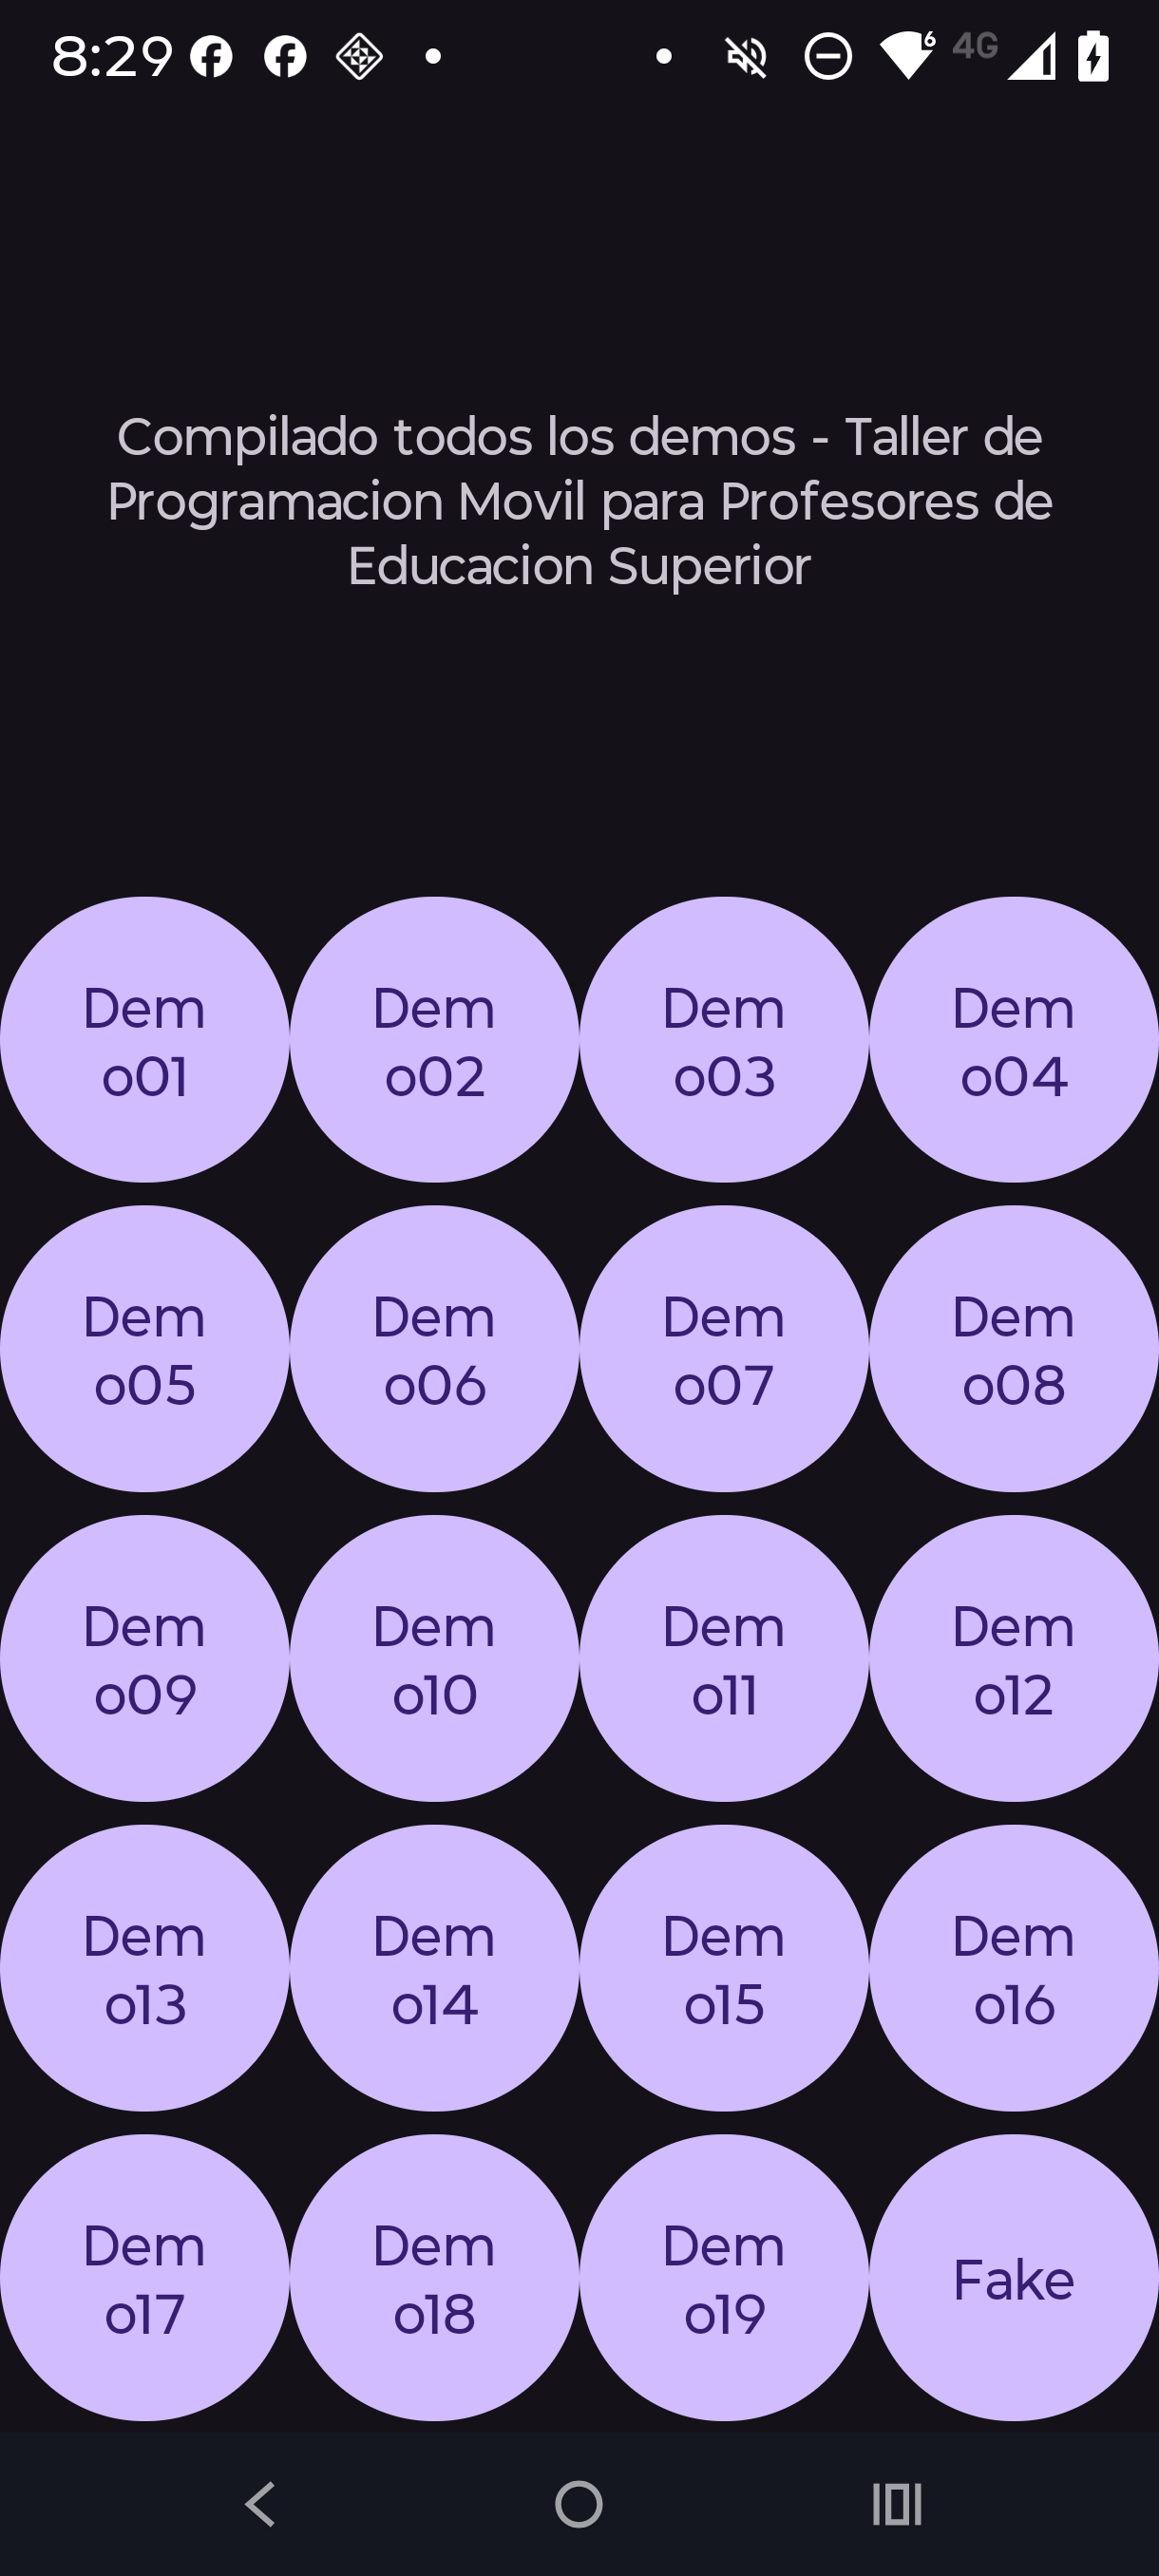
\includegraphics[width=0.98\textwidth]{02_TallerCBTis/figs/Demo20}
\end{center}

\end{columns}

\end{frame}

